\documentclass{article}
\usepackage[utf8]{inputenc}
\usepackage{lipsum}
\usepackage[left=2cm, right=2cm, top=3cm, includefoot]{geometry}
\usepackage{comment}
\usepackage {graphicx}%Import images
\usepackage{float}%Set any float position of images for example.
\usepackage{titlepic}
\usepackage{multirow}


\graphicspath{ {\Users\soren\Desktop\Projects 5. semester\Big Data/} }


%Allows for different colors in report
\usepackage{color}
\usepackage[dvipsnames, table, xcdraw]{xcolor}
\usepackage{tabu}
\usepackage{dcolumn}
\newcolumntype{A}{D{.}{.}{2.3}}
\setlength{\parindent}{0pt}


%Setup allows for clickable ToC with different colors
\usepackage{hyperref}
\hypersetup{
    colorlinks,
    citecolor=black,
    filecolor=black,
    linkcolor=black,
    urlcolor=black
}


% Header and Footer Stuff
\usepackage{fancyhdr}
\pagestyle{fancy} %Use fancy page style
\fancyhead[R]{CBS} %Align to the right on the page
\fancyfoot{}
\fancyfoot[R]{\thepage\ } %Align to the right on the page
\renewcommand{\headrulewidth}{0.5pt} %overwrite headers width
\renewcommand{\footrulewidth}{1pt}  %overwrite footers width




\begin{comment}
Renew command overwrites a previous function. Therefore, it is used to overwrite the header and footer width.
fancyfootHDR package, allows us to add cool headers and footers. R aligns to the right  \thepage\ references the actual page number.
\end{comment}




%
\begin{document}





%Start of titlepage
\begin{titlepage}
	\begin{center}
	\line(1,0){300} \\
	[0.25in]
	\color{NavyBlue} \huge{\bfseries A Big Data Research Paper} \\   
	[2mm]	
	\color{black}
	\line(1,0) {200} \\
	[0.1cm]
	\color{black}\textsc{\LARGE On Donald J. Trump's Twitter Activity} \\
	[0.75cm]
	\textsc{\LARGE Copenhagen Business School} \\
	[9.5cm]




\end{center}



\begin{figure}[H]
	\centering

%
 %\raisebox{20mm}[0pt][0pt]{
 %\makebox[\textwidth][c]{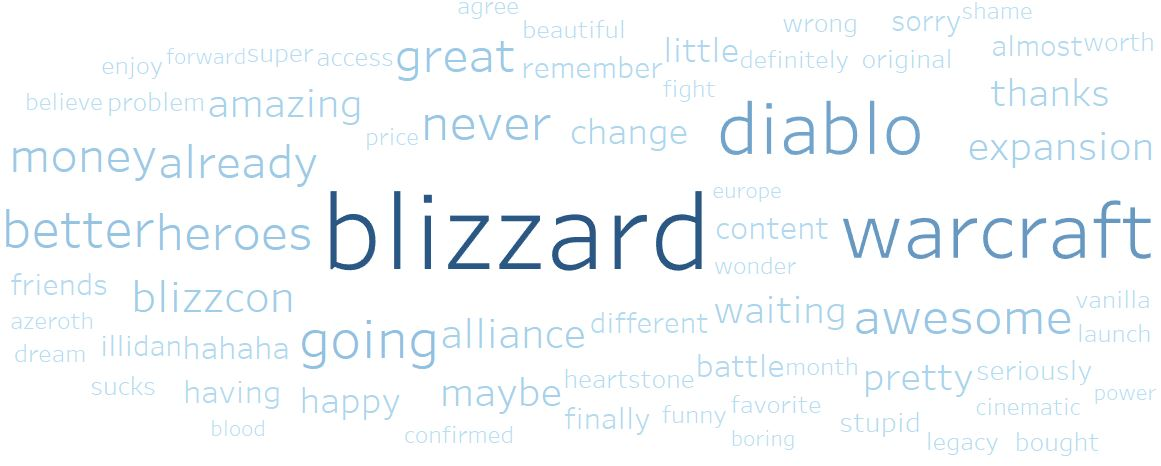
\includegraphics[scale=.55]{BlizzardWord2Cloud.PNG}
 %}}

\vspace*{-12cm} 
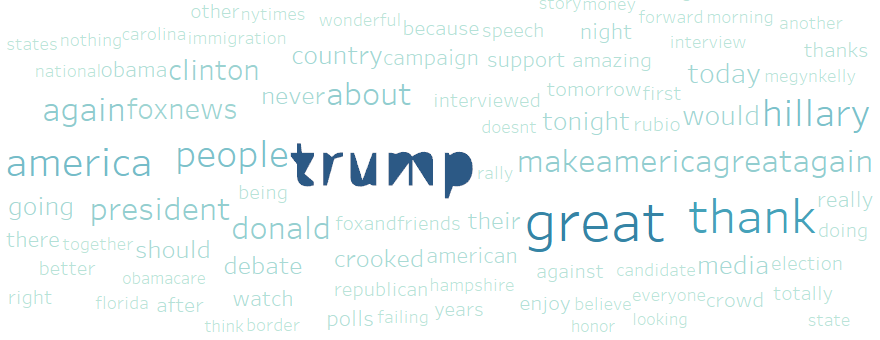
\includegraphics[scale=.75]{TrumpWord.PNG}



\caption{ Trump Wordcloud }
\vspace*{1.25cm} 


\end{figure}


	\begin{flushright}
\vspace*{1.25cm} 

	\textsc{\large Søren Kolbye Jensen \\}
	Bsc. Ha(IT) \\
	\#43124133123 \\
	December 1, 2017
	\end{flushright}





%End of titlepage
\end {titlepage}



%Table of contents & summary
\color{NavyBlue} \tableofcontents \color{black}
\thispagestyle{empty} %Remove the header, by removing all the style
 \cleardoublepage
\setcounter{page}{1}%Reset page counter at introduction page 
\pagenumbering{arabic}
%\addcontentsline{toc}{section}{\numberline{}Summary}


\cleardoublepage%Table of contents end


\section{Summary} %Summary
Summary section


\cleardoublepage %Summary end


%End of table of contents & summary









%Start of report






%Start of introduction_____________________________________________


\color{NavyBlue} \section{Introduction} \label{sec:intro}

\color {black}

Big Data has changed how data is viewed in society, businesses have  invested heavily in infrastructure that can imrpove data collection.
It is now possible, to use Big Data to analyze the behaviour of Social Media channels such as Twitter, Facebook and Instagram. 
However, the vast amount of data available with modern technologies has proven difficult to analyze. According to ??, Big Data can be either
structured or unstrucuted, where the determining parameters are "Velocity, Verocity and Validity". In order to surmount  this difficulty, new datamining technologies 
has been invented, in order to aid the field of Data Science. \\

These principles are called "Datascience and Datamining". According to (INSERT BOOK), datascience and datamining can be defined as follows: \\

Data science is the act of using fundamental principles, to guide extraction of knowledge from datasets. \\

Datamining on the other hand, deals with extracting knowledge from data using technolgoies, which incorporates the principles of data science.  \\

This research paper, aims to use the fundamental principles of Data science, in conjunction with  datamining technologies. 
To analyze the behvaiour of U.S president Donald J. Trump. and how this behaviour affected his political campaign, as well as how his behaviour affected the American financial markets.



%Big Data  book ch1


\begin{figure}[H] %We begin our figure and want it to stay H(ere)
	\centering %We want to center the figure
\fbox{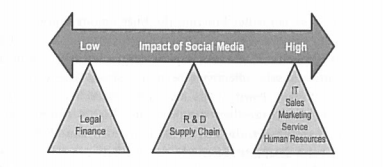
\includegraphics [scale= 1.25]  {Threefactor.PNG}    } %Include our ijmage with a height and location of img.
	\caption[Optional caption] {real, local caption for refrence}
	\label{fig:wordcloudBliz}

\end{figure}






\subsection{Case introduction}
Donald John Trump, born in 1946 in Queens New York, is the CEO of the Trump Organization and is well known as a real-estate broker in the United States.
However, on june 16th, 2015, Trump officially announced his candidacy as the 20th US President". This political campaign was heavily involved with Social Media, as Trump was actively fighting big news channels, such
as CNN, NBC etc. labelling them as "fake news". Thus, Trump figured out a way to distribute highly controversial statements and gain political support by his use of Social Media Channels such as Twitter. 


%http://secfilings.nasdaq.com/edgar_conv_html%2f2017%2f02%2f28%2f0001047469-17-001072.html#FIS_BUSINESS

\cleardoublepage



%End of introduction________________________________

%https://www.aol.com/2016-election/timeline/
%https://www.dropbox.com/sh/kd87npmrvcwiyge/AADRTmSB6lDt5ChunVY_Xy0Ea/ExampleProjects?dl=0&preview=ExampleProject%2301-VisualAnalytics-NYC_TaxiRides-GreenCabs_vs_Uber.pdf

\section{Problem Formulation and Reserach questions} \label{sec:ch1}
The goal of this research paper is to analyze  trumps behaviour on Twitter and how he used Twitter to combat "fake news". A visual analysis on his behaviour between DATE and DATE will be conducted to reveal the patterns in his behaviour in this timeframe. This leads to the reserach question: 

\par\vspace{10pt}

What was trump's behaviour on social media, prior to his announcement of his presidency. And how did it change, during and after his political campaign.\\

Furthermore, Trump's political campaign was heavily focused on combating illegal immigration. One of the primary targets of Trump's statement was Mexico.
This leads to the research question:

How did Trump's political statements on Twitter affect the American and Meixcan currency?


\section{Theoretical Framework}
For this research paper, an usupervised data mining technique has been chosen. With this method there are no pretetermined attirbutes or a specific target.
This research aims to use induction and deduction to find correlations among data. Thus revealing a structure, which was otherwhise hidden.

Clustering maybe? When distributing fake news and stuff? idk \\ (Reveal groups and categories, previously unaware of) -> Further datamining discover new correlations

Association: Co-occurences among events. -> Example, Trump becomes president and the currency falls, why?
Asosciation rules "50 percent of the activity is negative?" \\

Feature extraction: If violense, action, heroism is an attribute of a film then "action" may be trhe feature. 
You can say that news can have t he feature fake or real?\\



%https://cloudtweaks.com/2014/09/use-supervised-unsupervised-data-mining/

%Methodology start

\section{Methodology}
To answer the research questions two different types of analysis is presented\\


Furthermore,  the CRISP framework has been used in a modified fashion, in order to better illustrate the context of this research paper.\\

\begin{figure}[H] %We begin our figure and want it to stay H(ere)
	\centering %We want to center the figure
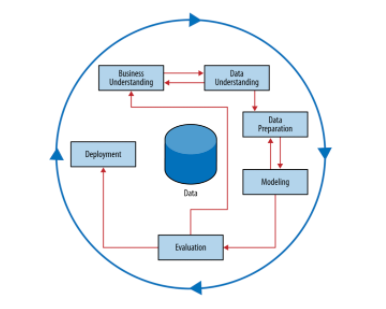
\includegraphics [scale= .95]  {CRISP.PNG}    %Include our ijmage with a height and location of img.
	\caption[Optional caption] {real, local caption for refrence}
	\label{fig:wordcloudBliz}

\end{figure}


The model serves to illustrate how the data was processed throughout the proejct in order to yield a final result/answer to the resarch questions. The model is iterative and serves to explore the Twitter data, so a better
understanding of the data can be reached. This process has been conciously iterated throughout the project.

"Business understanding" is in this context the overall problem formulation and research questions that we wish answered.\\
For every iteration a deeper understanding of the data is achieved, which affects the understanding of the overall research framework.

"Data preperation" is where we merge, cleanse and integrate multiple data sources. In this research paper, Alteryx has been used as shown in Table 1 later in the report.
"Modelling has used Tableau, which is a visual analytics tool. This makes it easier to explore and understand the patterns presented in the data.

"Evaluation" Here we evaluate, whether the data model that has been built answers the overall research questions. After the model has been evaluated and validated, the model will go through "deployment", which in this sense will be the final conclusion to
the research questions.\\
















%Table
%https://www.alteryx.com/analytics/data-mining-software

%Data Analytics tool that provide data mining solutions
% by helping with data cleansing and integration 
%of multiple sources.
%This tool helps with visual data representations in a 
%dynamic environment, where several datasets can be
%joined in order to create a comprehensive data solution.
 To summarize, Table 1 shows the purpose and use of each datamining tool used in this research paper: 


\begin{table}[H]
\centering
\caption{My caption}
\label{my-label}
\begin{tabular}{|l|l|l|l|l|}
\hline
\rowcolor[HTML]{656565} 
{\color[HTML]{000000} \textbf{Tool:}} & {\color[HTML]{000000} \textbf{Purpose:}} & \multicolumn{3}{l|}{\cellcolor[HTML]{656565}{\color[HTML]{000000} \textbf{Use:}}} \\ \hline
\rowcolor[HTML]{BBDAFF} 
\cellcolor[HTML]{BBDAFF}{\color[HTML]{000000} } & \cellcolor[HTML]{BBDAFF}{\color[HTML]{000000} } & \multicolumn{3}{l|}{\cellcolor[HTML]{BBDAFF}{\color[HTML]{000000} }} \\
\rowcolor[HTML]{BBDAFF} 
\cellcolor[HTML]{BBDAFF}{\color[HTML]{000000} } & \cellcolor[HTML]{BBDAFF}{\color[HTML]{000000} } & \multicolumn{3}{l|}{\cellcolor[HTML]{BBDAFF}{\color[HTML]{000000} }} \\
\rowcolor[HTML]{BBDAFF} 
\multirow{-3}{*}{\cellcolor[HTML]{BBDAFF}{\color[HTML]{000000} \textbf{Alteryx}}} & \multirow{-3}{*}{\cellcolor[HTML]{BBDAFF}{\color[HTML]{000000} \begin{tabular}[c]{@{}l@{}}Data Analytics tool that \\ provide data mining solutions\\  by helping with data \\ cleansing and integration \\ of multiple sources.\end{tabular}}} & \multicolumn{3}{l|}{\multirow{-3}{*}{\cellcolor[HTML]{BBDAFF}{\color[HTML]{000000} \begin{tabular}[c]{@{}l@{}}Lorem ipsumLorem ipsumLorem \\ ipsumLorem ipsum\\ Lorem ipsumLorem ipsumLorem ipsum\end{tabular}}}} \\ \hline
\rowcolor[HTML]{BBDAFF} 
\cellcolor[HTML]{BBDAFF}{\color[HTML]{000000} } & \cellcolor[HTML]{BBDAFF}{\color[HTML]{000000} } & \multicolumn{3}{l|}{\cellcolor[HTML]{BBDAFF}{\color[HTML]{000000} }} \\
\rowcolor[HTML]{BBDAFF} 
\cellcolor[HTML]{BBDAFF}{\color[HTML]{000000} } & \cellcolor[HTML]{BBDAFF}{\color[HTML]{000000} } & \multicolumn{3}{l|}{\cellcolor[HTML]{BBDAFF}{\color[HTML]{000000} }} \\
\rowcolor[HTML]{BBDAFF} 
\multirow{-3}{*}{\cellcolor[HTML]{BBDAFF}{\color[HTML]{000000} \textbf{Tableau}}} & \multirow{-3}{*}{\cellcolor[HTML]{BBDAFF}{\color[HTML]{000000} \begin{tabular}[c]{@{}l@{}}This tool helps with visual\\ data representation.\end{tabular}}} & \multicolumn{3}{l|}{\multirow{-3}{*}{\cellcolor[HTML]{BBDAFF}{\color[HTML]{000000} \begin{tabular}[c]{@{}l@{}}Lorem ipsumLorem ipsumLore\\ m iLorem ipsumpsumdasdLo\\ remLorem ipsum ipsum\end{tabular}}}} \\ \hline
\end{tabular}
\end{table}


\subsection{Data Acquisition and Dataset Description}
The datasets in this research paper has been collected from Trump's Twitter page, ranging from 2009 to 2017.

The first datasets consists of Twitter data on Trump's primary twitter channel.  This dataset will mainly be used to analyze Trump and his Campaign team's behaivour. 

The second dataset consists of Historical data on the American and Mexican currency between Trump's announcement to  14/07/2017

The third dataset is collected through Sentione and will be used to analyze the sentiment towards Trump's campaign. Ranging from before his inagruation, until 02/11/2017. 

\cleardoublepage



%End of report__________________________________



\end{document}






%\begin{figure}[H] %We begin our figure and want it to stay H(ere)
%	\centering %We want to center the figure


 %\raisebox{10mm}[0pt][0pt]{
%\fbox{ \makebox[\textwidth][c]{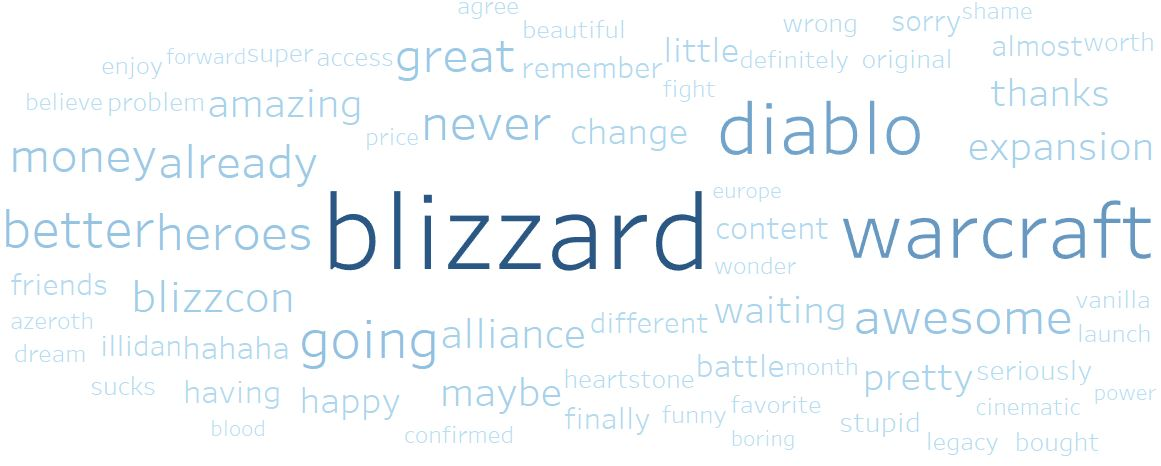
\includegraphics[scale=.55]{BlizzardWord2Cloud.PNG}}
% }}
%\vspace*{-40mm} %Close in the caption to the image

%\protect\caption[position=bottom]{Title of Figure\label{fig:F1}}


%\vspace{3cm}
%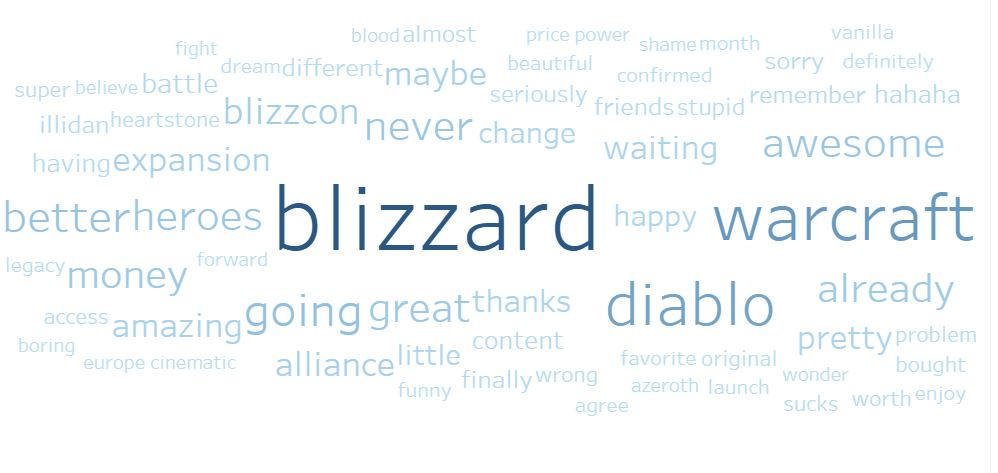
\includegraphics [width = 7in]  {BlizzardWordCloud.PNG}     %Include our ijmage with a height and location of img.
	
%	\label{fig:wordcloudBliz}

%\end{figure}



